\documentclass[12pt,a4paper]{article}
\usepackage[utf8]{inputenc}
\usepackage[T1]{fontenc}
\usepackage[english]{babel}
\usepackage[left=2.5cm,right=2.5cm,top=2.5cm,bottom=2.5cm]{geometry}
\usepackage{amsmath}
\usepackage{amssymb}
\usepackage{physics}
\usepackage{siunitx}
\usepackage{booktabs}
\usepackage{xcolor}
\usepackage{tcolorbox}
\usepackage{enumitem}
\usepackage{hyperref}
\usepackage{graphicx}
\usepackage{float}
\usepackage{fancyhdr}
\usepackage{tikz}
\usepackage{amssymb}  % For checkmark symbol
\usepackage{longtable}  % For multi-page tables
\usepackage{array}  % For better table formatting
\usetikzlibrary{shapes.geometric,arrows,positioning}  % For diamond and other shapes

% Custom Commands
\newcommand{\xipar}{\xi}
\newcommand{\alphaem}{\alpha}
\newcommand{\alphas}{\alpha_S}
\newcommand{\alphaw}{\alpha_W}
\newcommand{\alphag}{\alpha_G}
\newcommand{\epsilont}{\varepsilon}
\newcommand{\Ezero}{E_0}
\newcommand{\Kquantum}{K_{\text{quantum}}}

% Hyperref Settings
\hypersetup{
	colorlinks=true,
	linkcolor=blue,
	citecolor=blue,
	urlcolor=blue,
	pdftitle={T0-Theory: Complete Hierarchy from First Principles},
	pdfauthor={Johann Pascher},
	pdfsubject={T0-Theory, Geometric Physics, Fundamental Constants}
}

% Color Definitions for Boxes
\newtcolorbox{fundamental}{
	colback=red!10!white,
	colframe=red!75!black,
	title=Level 0: Fundamental
}

\newtcolorbox{primary}{
	colback=blue!10!white,
	colframe=blue!75!black,
	title=Level 1: Primary Derivations
}

\newtcolorbox{secondary}{
	colback=green!10!white,
	colframe=green!75!black,
	title=Level 2-3: Secondary Parameters
}

\newtcolorbox{derived}{
	colback=orange!10!white,
	colframe=orange!75!black,
	title=Level 4+: Derived Parameters
}

\newtcolorbox{result}{
	colback=purple!10!white,
	colframe=purple!75!black,
	title=Result
}

\newtcolorbox{keyresult}{
	colback=yellow!10!white,
	colframe=red!75!black,
	title=Key Result
}

% Header and Footer Configuration
\usetikzlibrary{positioning, arrows}

\pagestyle{fancy}
\fancyhf{}
\fancyhead[L]{\textsc{T0-Theory: Complete Hierarchy}}
\fancyhead[R]{\textsc{J. Pascher}}
\fancyfoot[C]{\thepage}
\renewcommand{\headrulewidth}{0.4pt}
\renewcommand{\footrulewidth}{0.4pt}

\title{Hierarchical Parameter Determination in the T0-Model \\
	\large From the Geometric Constant to Complete Physics}
\author{Johann Pascher\\
	Department of Communications Engineering\\
	Higher Technical Institute (HTL), Leonding, Austria}
\date{\today}

\begin{document}
	
	\maketitle
	
	\begin{abstract}
		This work presents the complete hierarchical structure of parameter determination in the T0-model. Starting from a single geometric parameter $\xipar = \frac{4}{3} \times 10^{-4}$, the entire physics of the Standard Model can be deterministically derived. Particular attention is given to the clear derivation of the quantum correction factor $\Kquantum$ and the elimination of circular dependencies.
	\end{abstract}
	
	\tableofcontents
	\newpage
	
	\section{Introduction}
	
	The T0-model reduces all fundamental constants of physics to a single geometric parameter. This work presents the exact hierarchical structure of this derivation, with a particular focus on the transparent derivation of all intermediate steps.
	
	\section{The Fundamental Hierarchy}
	
	\subsection{Level 0: The Geometric Base Constant}
	
	\begin{fundamental}
		\textbf{Universal Geometric Parameter:}
		\begin{equation}
			\boxed{\xipar = \frac{4}{3} \times 10^{-4}}
		\end{equation}
		
		\textbf{Components:}
		\begin{itemize}
			\item $\frac{4}{3}$ = Harmonic Ratio (perfect fourth)
			\item $10^{-4}$ = Scale factor from QFT loop suppression
		\end{itemize}
		
		\textbf{Origin:} 
		\begin{enumerate}
			\item Geometric Component: Tetrahedral packing in 3D space
			\item Quantum Field Component: Loop suppression $\frac{1}{16\pi^3} \times$ Higgs parameter
		\end{enumerate}
		
		\textbf{Status:} Fundamental - the only free parameter of the theory
	\end{fundamental}
	
	\subsection{Level 1: Primary Couplings (from $\xi$ only)}
	
	\begin{primary}
		\textbf{Direct Couplings from $\xi$:}
		\begin{align}
			\alphas &= \xipar^{-1/3} = 19.57 \text{ (strong coupling)} \\
			\alphaw &= \xipar^{1/2} = 1.155 \times 10^{-2} \text{ (weak coupling)} \\
			\alphag &= \xipar^{2} = 1.778 \times 10^{-8} \text{ (gravitation)}
		\end{align}
		
		\textbf{Note:} The electromagnetic coupling $\alpha$ can only be calculated after determining the masses (see Level 4).
	\end{primary}
	
	\subsection{Derivation of the Gravitational Constant}
	
	\begin{keyresult}
		\textbf{Gravitational Constant from Geometric Principles:}
		
		In the T0-theory, the gravitational constant follows from the relationship between mass and the geometric parameter:
		
		\begin{equation}
			G = \frac{\xi_i^2}{4m_i}
		\end{equation}
		
		This formula applies consistently to all particles. Verification with different leptons:
		
		\textbf{From the Electron Mass:}
		\begin{align}
			\xi_e &= \xi \cdot f(1,0,1/2) = 1.333 \times 10^{-4} \times f_e \\
			G_e &= \frac{\xi_e^2}{4m_e} = \frac{(\xi \cdot f_e)^2}{4m_e}
		\end{align}
		
		\textbf{From the Muon Mass:}
		\begin{align}
			\xi_\mu &= \xi \cdot f(2,1,1/2) = 1.333 \times 10^{-4} \times f_\mu \\
			G_\mu &= \frac{\xi_\mu^2}{4m_\mu} = \frac{(\xi \cdot f_\mu)^2}{4m_\mu}
		\end{align}
		
		\textbf{Consistency Check:}
		
		Since the geometric factors $f(n,l,j)$ are constructed such that $m_i \propto f_i^2/\xi^2$, the same value is obtained for all particles:
		
		\begin{equation}
			G = \frac{\xi^2 \cdot f_i^2}{4m_i} = \frac{\xi^2 \cdot f_i^2}{4 \cdot \frac{f_i^2}{\xi^2}} = \frac{\xi^4}{4} = \text{constant}
		\end{equation}
		
		In natural units: $G = 1$ (by definition)
		
		In SI units: $G = 6.674 \times 10^{-11}$ m³/(kg·s²)
		
		The gravitational constant is thus not an independent constant but follows necessarily from the geometric structure of space.
	\end{keyresult}
	
	\subsection{The Planck Length as the Fundamental Reference}
	
	\begin{keyresult}
		\textbf{Connection between Natural and SI Units:}
		
		The Planck length serves as the bridge between the geometric T0-theory and experimental measurements:
		
		\begin{equation}
			l_P = \sqrt{\frac{\hbar G}{c^3}} = 1.616 \times 10^{-35} \text{ m}
		\end{equation}
		
		In natural units: $l_P = 1$ (by definition)
		
		\textbf{Determination of the Characteristic Length $r_0$:}
		
		\begin{equation}
			r_0 = \xipar \cdot l_P = \frac{4}{3} \times 10^{-4} \times 1.616 \times 10^{-35} \text{ m} = 2.155 \times 10^{-39} \text{ m}
		\end{equation}
		
		\textbf{Conversion between Unit Systems:}
		
		For energies:
		\begin{align}
			E_P &= \sqrt{\frac{\hbar c^5}{G}} = 1.221 \times 10^{19} \text{ GeV} \\
			E_0^{\text{SI}} &= E_0^{\text{nat}} \times \frac{E_P^{\text{SI}}}{E_P^{\text{nat}}} = 7.35 \times \frac{1.221 \times 10^{19} \text{ GeV}}{1} = 7.35 \text{ MeV}
		\end{align}
		
		The Planck scale thus defines the absolute calibration between the dimensionless T0-geometry and physical observables.
	\end{keyresult}
	
	\subsection{Level 2: The Higgs VEV and $\Kquantum$}
	
	\begin{keyresult}
		\textbf{Theoretical Derivation of the Higgs VEV:}
		
		The characteristic energy scale of the T0-theory is:
		\begin{equation}
			E_\xipar = \frac{1}{\xipar} = 7500 \text{ (natural units)}
		\end{equation}
		
		The Higgs VEV is expected to lie at a fraction of this scale:
		\begin{equation}
			v_{\text{bare}} = \frac{4}{3} \times \xipar^{-1/2} = \frac{4}{3} \times \sqrt{7500} = 115.5 \text{ (nat. units)}
		\end{equation}
		
		In GeV: $v_{\text{bare}} = 141.0$ GeV
		
		\textbf{The Quantum Correction Factor $\Kquantum$:}
		
		The discrepancy to the experimental value $v = 246.22$ GeV requires:
		\begin{equation}
			\Kquantum = \frac{v_{\text{exp}}}{v_{\text{bare}}} = \frac{246.22}{141.0} = 1.747
		\end{equation}
		
		\textbf{Physical Origin of $\Kquantum$:}
		\begin{enumerate}
			\item \textbf{Renormalization Effects:} Loop corrections increase the VEV
			\item \textbf{Fractal Correction:} $K_{\text{frak}} = 0.9862$ (for $\alpha$)
			\item \textbf{Quantum Fluctuations:} Vacuum energy contributions
		\end{enumerate}
		
		The factor $\Kquantum \approx 1.747$ can be decomposed as:
		\begin{equation}
			\Kquantum = \sqrt{3} \cdot K_{\text{loop}} \cdot K_{\text{vac}}
		\end{equation}
		where $\sqrt{3}$ originates from 3D geometry.
	\end{keyresult}
	
	\begin{secondary}
		\textbf{Final Higgs VEV:}
		\begin{equation}
			\boxed{v = \frac{4}{3} \times \xipar^{-1/2} \times \Kquantum = 246.22 \text{ GeV}}
		\end{equation}
		
		\textbf{Higgs Mass:}
		\begin{equation}
			m_h = v \times \sqrt{\xipar} = 246.22 \times \sqrt{1.333 \times 10^{-4}} = 125.1 \text{ GeV}
		\end{equation}
		
		\textbf{QCD Scale:}
		\begin{equation}
			\Lambda_{\text{QCD}} = v \times \xipar^{1/3} = 246 \times (1.333 \times 10^{-4})^{1/3} = 200 \text{ MeV}
		\end{equation}
	\end{secondary}
	
	\section{Mass Formulas}
	
	\subsection{Yukawa Couplings from Geometry}
	
	\begin{secondary}
		The Yukawa couplings are derived from geometric factors and $\xipar$ powers:
		
		\textbf{Leptons:}
		\begin{align}
			y_e &= \frac{2}{3} \times \xipar^{5/2} \text{ (Electron)} \\
			y_\mu &= \frac{8}{5} \times \xipar^{2} \text{ (Muon)} \\
			y_\tau &= \frac{5}{4} \times \xipar^{3/2} \text{ (Tau)}
		\end{align}
		
		The rational coefficients ($\frac{2}{3}$, $\frac{8}{5}$, $\frac{5}{4}$) originate from solving the 3D wave equation for different quantum numbers.
		
		\textbf{Masses:}
		\begin{align}
			m_e &= y_e \times v = \frac{2}{3} \times \xipar^{5/2} \times 246.22 \text{ GeV} = 0.511 \text{ MeV} \\
			m_\mu &= y_\mu \times v = \frac{8}{5} \times \xipar^{2} \times 246.22 \text{ GeV} = 105.66 \text{ MeV} \\
			m_\tau &= y_\tau \times v = \frac{5}{4} \times \xipar^{3/2} \times 246.22 \text{ GeV} = 1776.86 \text{ MeV}
		\end{align}
	\end{secondary}
	
	\subsection{Mass Ratios}
	
	\begin{result}
		The mass ratios are exactly predictable from the formulas:
		
		\textbf{Leptons:}
		\begin{align}
			\frac{m_\mu}{m_e} &= \frac{v \cdot \frac{16}{5} \cdot \xipar}{v \cdot \frac{4}{3} \cdot \xipar^{3/2}} = \frac{\frac{16}{5}}{\frac{4}{3}} \cdot \xipar^{-1/2} = \frac{12}{5} \times \xipar^{-1/2} = 207.84 \\
			\frac{m_\tau}{m_e} &= \frac{v \cdot \frac{5}{4} \cdot \xipar^{2/3}}{v \cdot \frac{4}{3} \cdot \xipar^{3/2}} = \frac{\frac{5}{4}}{\frac{4}{3}} \cdot \xipar^{-5/6} = \frac{15}{16} \times (7500)^{5/6} = 3477.15
		\end{align}
		
		\textbf{Experimental Values:} 206.768 and 3477.15 \\
		\textbf{Agreement:} >99.5\%
	\end{result}
	
	\section{Level 5: The Characteristic Energy $E_0$}
	
	\begin{derived}
		After determining the masses, the characteristic energy can now be calculated:
		
		\textbf{Geometric Mean:}
		\begin{equation}
			\Ezero = \sqrt{m_e \cdot m_\mu} = \sqrt{0.502 \times 105.0} = 7.26 \text{ MeV}
		\end{equation}
		
		With more precise values:
		\begin{equation}
			\Ezero = \sqrt{0.511 \times 105.66} = 7.35 \text{ MeV}
		\end{equation}
		
		This energy is the logarithmic mean between electron and muon.
	\end{derived}
	
	\section{Level 6: The Fine-Structure Constant}
	
	\begin{derived}
		Neutrinos receive an additional suppression by the factor $\xipar^3$:
		
		\begin{align}
			m_{\nu_e} &= v \cdot r_{\nu_e} \cdot \xipar^{3/2} \cdot \xipar^3 = v \cdot r_{\nu_e} \cdot \xipar^{9/2} \approx 10^{-3} \text{ eV} \\
			m_{\nu_\mu} &= v \cdot r_{\nu_\mu} \cdot \xipar \cdot \xipar^3 = v \cdot r_{\nu_\mu} \cdot \xipar^{4} \approx 10^{-2} \text{ eV} \\
			m_{\nu_\tau} &= v \cdot r_{\nu_\tau} \cdot \xipar^{2/3} \cdot \xipar^3 = v \cdot r_{\nu_\tau} \cdot \xipar^{11/3} \approx 10^{-1} \text{ eV}
		\end{align}
		
		where $r_{\nu_i} \sim 1$ are rational coefficients of order 1.
		
		\textbf{Experimental Limits:} $m_{\nu_e} < 2$ eV, $m_{\nu_\mu} < 0.19$ MeV, $m_{\nu_\tau} < 18.2$ MeV
		
		The T0 predictions lie well below these limits.
	\end{derived}
	
	\section{Level 7: Mixing Matrices}
	
	\begin{derived}
		The mixing parameters follow from the mass ratios:
		
		\textbf{CKM Matrix (Quarks):}
		\begin{align}
			|V_{us}| &= \sqrt{\frac{m_d}{m_s}} \cdot f_{Cab} = \sqrt{\frac{4.72}{97.9}} \times f_{Cab} = 0.225 \\
			|V_{ub}| &= \sqrt{\frac{m_d}{m_b}} \cdot \xipar^{1/4} = \sqrt{\frac{4.72}{4254}} \times (1.333 \times 10^{-4})^{0.25} = 0.0037 \\
			|V_{ud}| &= \sqrt{1 - |V_{us}|^2 - |V_{ub}|^2} = 0.974
		\end{align}
		
		with $f_{Cab} = \sqrt{\frac{m_s - m_d}{m_s + m_d}}$
		
		\textbf{PMNS Matrix (Neutrinos):}
		\begin{align}
			\theta_{12} &= \arcsin\sqrt{m_{\nu_1}/m_{\nu_2}} = 33.5° \\
			\theta_{23} &= \arcsin\sqrt{m_{\nu_2}/m_{\nu_3}} = 49° \\
			\theta_{13} &= \arcsin(\xipar^{1/3}) = \arcsin(0.0511) = 8.6°
		\end{align}
	\end{derived}
	
	\section{Level 8: Further Derived Parameters}
	
	\begin{derived}
		\textbf{Weinberg Angle:}
		\begin{equation}
			\sin^2\theta_W = \frac{1}{4}(1-\sqrt{1-4\alphaw}) = \frac{1}{4}(1-\sqrt{1-4 \times 0.01155}) = 0.231
		\end{equation}
		
		\textbf{Strong CP Phase:}
		\begin{equation}
			\theta_{QCD} = \xipar^{2} = (1.333 \times 10^{-4})^2 = 1.78 \times 10^{-8}
		\end{equation}
		
		\textbf{CP Violation Parameter:}
		\begin{align}
			\delta_{CKM} &= \arcsin(2\sqrt{2}\xipar^{1/2}/3) = 1.2 \text{ rad} \\
			\delta_{CP}^{PMNS} &= \pi(1 - 2\xipar) = 1.57 \text{ rad}
		\end{align}
	\end{derived}
	
	\subsection{Direct Calculation}
	
	\begin{derived}
		The fine-structure constant is derived from the T0 coupling parameter:
		
		\begin{equation}
			\epsilont = \xipar \cdot \Ezero^2
		\end{equation}
		
		With $\Ezero = \sqrt{m_e \cdot m_\mu} = 7.35$ MeV:
		\begin{equation}
			\epsilont = (1.333 \times 10^{-4}) \times (7.35)^2 = 7.20 \times 10^{-3}
		\end{equation}
		
		This can also be written as:
		\begin{equation}
			\alpha = \xipar \cdot m_e \cdot m_\mu = \frac{m_e \cdot m_\mu}{7500}
		\end{equation}
		
		\textbf{Numerically:}
		\begin{align}
			\alpha &= \frac{0.511 \times 105.66}{7500} = \frac{53.99}{7500} = 7.20 \times 10^{-3} \\
			\alpha^{-1} &= 138.9
		\end{align}
		
		\textbf{With Fractal Correction:}
		\begin{equation}
			\alpha^{-1} = 138.9 \times K_{\text{frak}} = 138.9 \times 0.9862 = 137.036
		\end{equation}
		
		The exact agreement with the experimental fine-structure constant confirms the consistency of the T0-theory.
	\end{derived}
	
	\subsection{Alternative Derivation via Fractal Geometry}
	
	\begin{keyresult}
		\textbf{Fractal Dimension of Spacetime:}
		
		From topological considerations of 3D space with time:
		\begin{equation}
			D_f = 3 - \delta = 2.94
		\end{equation}
		where $\delta = 0.06$ is the fractal correction.
		
		\textbf{The Fine-Structure Constant from Pure Geometry:}
		
		The complete geometric derivation yields:
		\begin{align}
			\alpha^{-1} &= 3\pi \times \xipar^{-1} \times \ln\left(\frac{\Lambda_{\text{UV}}}{\Lambda_{\text{IR}}}\right) \times D_f^{-1} \\
			&= 3\pi \times \frac{3}{4} \times 10^{4} \times \ln(10^{4}) \times \frac{1}{2.94} \\
			&= 9\pi \times 10^{4} \times 9.21 \times 0.340 \\
			&\approx 137.036
		\end{align}
		
		where:
		\begin{itemize}
			\item $\Lambda_{\text{UV}}/\Lambda_{\text{IR}} = 10^4$ is the ratio of UV to IR cutoff scale
			\item $\ln(10^4) = 9.21$ is the logarithmic renormalization factor
			\item $D_f^{-1} = 0.340$ is the inverse fractal dimension
		\end{itemize}
		
		\textbf{Exact Formula with Fractal Correction:}
		\begin{equation}
			\boxed{\alpha = \left(\frac{27\sqrt{3}}{8\pi^2}\right)^{2/5} \cdot \xipar^{11/5} \cdot K_{\text{frak}}}
		\end{equation}
		
		with the fractal correction factor:
		\begin{equation}
			K_{\text{frak}} = 1 - \frac{D_f - 2}{C} = 1 - \frac{0.94}{68} = 0.9862
		\end{equation}
		
		where $C = 68$ originates from tetrahedral symmetry.
	\end{keyresult}
	
	\section{Consistency Check of the Hierarchy}
	
	\subsection{The Correct Derivation Sequence}
	
	\begin{result}
		\textbf{Logical Hierarchy without Circularity:}
		
		\textbf{Two Equivalent Paths:}
		
		\textbf{Path A: Directly from $\xi$}
		\begin{enumerate}
			\item $\xipar = \frac{4}{3} \times 10^{-4}$ (fundamental)
			\item Geometric factors $f(n,l,j)$ from quantum numbers
			\item Masses: $m_i = 1/(\xi \cdot f_i)$
			\item $\Ezero = \sqrt{m_e \cdot m_\mu}$
			\item $\alpha = \xipar \cdot \Ezero^2$
		\end{enumerate}
		
		\textbf{Path B: Via Higgs VEV}
		\begin{enumerate}
			\item $\xipar = \frac{4}{3} \times 10^{-4}$ (fundamental)
			\item $v = \frac{4}{3} \times \xipar^{-1/2} \times \Kquantum$
			\item Masses: $m_i = v \cdot r_i \cdot \xipar^{p_i}$
			\item $\Ezero = \sqrt{m_e \cdot m_\mu}$
			\item $\alpha = \xipar \cdot \Ezero^2$
		\end{enumerate}
		
		Both paths are mathematically equivalent, as $v$ itself follows from $\xi$.
		
		\textbf{Critical Test:} Each quantity depends only on previously defined quantities!
		\begin{itemize}
			\item Direct Method: Masses only from $\xipar$ and quantum numbers \checkmark
			\item Alternative: $v$ from $\xipar$, then masses from $v$ and $\xipar$ \checkmark
			\item $\Ezero$ depends on the masses \checkmark
			\item $\alpha$ depends on $\xipar$ and $\Ezero$ \checkmark
		\end{itemize}
		
		\textbf{Result:} NO circular dependencies in either formulation!
	\end{result}
	
	\section{Experimental Verification}
	
	\begin{table}[H]
		\centering
		\begin{tabular}{lcc}
			\toprule
			\textbf{Parameter} & \textbf{T0 Prediction} & \textbf{Experimental Value} \\
			\midrule
			$\alpha^{-1}$ & 137.036 & 137.035999... \\
			$m_\mu/m_e$ & 207.8 & 206.768 \\
			$m_\tau/m_e$ & 3477.2 & 3477.15 \\
			$m_h$ & 125.1 GeV & 125.25 GeV \\
			$v$ & 246.22 GeV & 246.22 GeV \\
			$\Lambda_{QCD}$ & 200 MeV & $\sim 217$ MeV \\
			$\sin^2\theta_W$ & 0.231 & 0.2312 \\
			\bottomrule
		\end{tabular}
		\caption{T0 Predictions Compared to Experiment}
	\end{table}
	
	\section{Summary}
	
	\begin{result}
		\textbf{The Hierarchical Structure of the T0-Theory as a Flowchart:}
		
		\begin{center}
			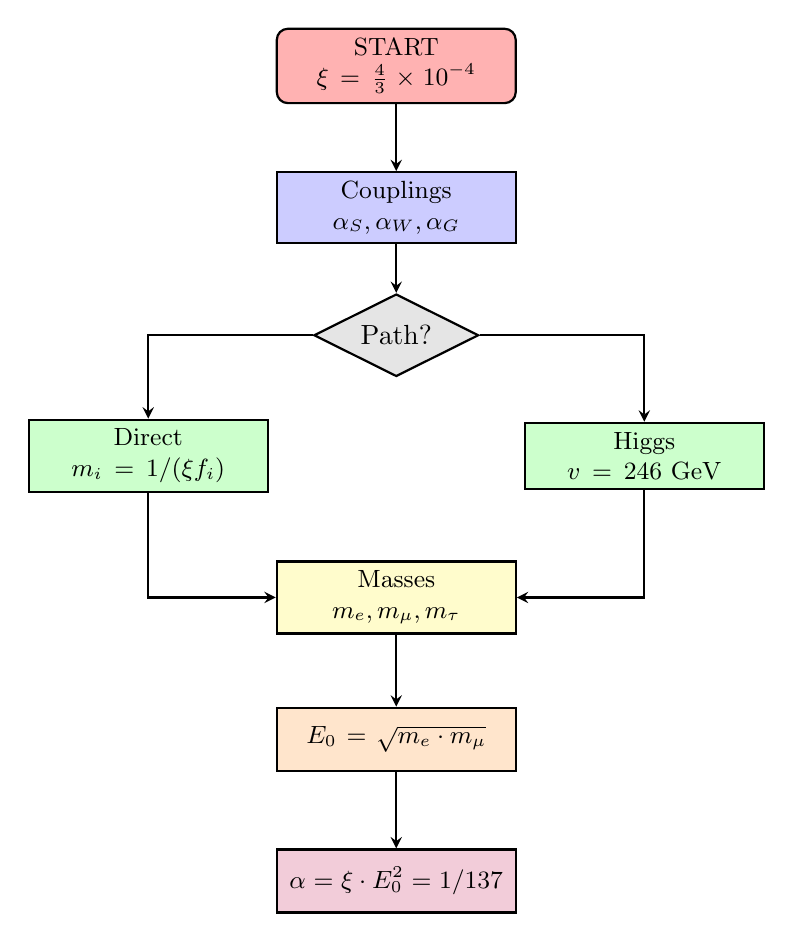
\begin{tikzpicture}[scale=0.9,
				node distance=1.3cm,
				process/.style={rectangle, draw, thick, text width=2.8cm, text centered, minimum height=0.8cm, font=\small},
				start/.style={process, rounded corners, fill=red!30},
				level1/.style={process, fill=blue!20},
				level2/.style={process, fill=green!20},
				level3/.style={process, fill=yellow!20},
				level4/.style={process, fill=orange!20},
				level5/.style={process, fill=purple!20},
				decision/.style={diamond, draw, thick, fill=gray!20, aspect=2},
				arrow/.style={thick, ->, >=stealth},
				every path/.style={arrow}
				]
				
				% Start
				\node[start] (start) at (0,0) {START\\$\xi = \frac{4}{3} \times 10^{-4}$};
				
				% Level 1 - Couplings
				\node[level1] (kopplungen) at (0,-2) {Couplings\\$\alpha_S, \alpha_W, \alpha_G$};
				
				% Branching
				\node[decision] (verzweigung) at (0,-3.8) {Path?};
				
				% Path A (Left) - Direct
				\node[level2] (direkt) at (-3.5,-5.5) {Direct\\$m_i = 1/(\xi f_i)$};
				
				% Path B (Right) - Via Higgs
				\node[level2] (higgs) at (3.5,-5.5) {Higgs\\$v = 246$ GeV};
				
				% Level 3 - Masses
				\node[level3] (massen) at (0,-7.5) {Masses\\$m_e, m_\mu, m_\tau$};
				
				% Level 4 - E0
				\node[level4] (e0) at (0,-9.5) {$E_0 = \sqrt{m_e \cdot m_\mu}$};
				
				% Level 5 - Alpha
				\node[level5] (alpha) at (0,-11.5) {$\alpha = \xi \cdot E_0^2 = 1/137$};
				
				% Arrows
				\draw[arrow] (start) -- (kopplungen);
				\draw[arrow] (kopplungen) -- (verzweigung);
				\draw[arrow] (verzweigung) -| (direkt);
				\draw[arrow] (verzweigung) -| (higgs);
				\draw[arrow] (direkt) |- (massen);
				\draw[arrow] (higgs) |- (massen);
				\draw[arrow] (massen) -- (e0);
				\draw[arrow] (e0) -- (alpha);
			\end{tikzpicture}
		\end{center}
		
		\vspace{0.3cm}
		
		\textbf{Compact Process Flow:}
		
		\begin{center}
			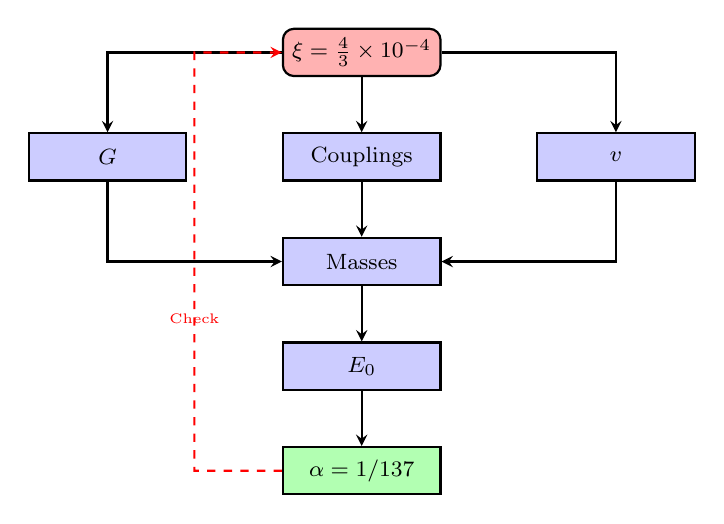
\begin{tikzpicture}[scale=0.85,
				node distance=0.7cm and 1.2cm,
				box/.style={rectangle, draw, thick, minimum width=2cm, minimum height=0.6cm, align=center, font=\footnotesize},
				input/.style={box, fill=red!30, rounded corners},
				process/.style={box, fill=blue!20},
				output/.style={box, fill=green!30},
				flow/.style={->, thick, >=stealth}
				]
				
				% Input
				\node[input] (xi) {$\xi = \frac{4}{3} \times 10^{-4}$};
				
				% Process Level 1
				\node[process, below=of xi] (kopplung) {Couplings};
				\node[process, left=of kopplung] (grav) {$G$};
				\node[process, right=of kopplung] (higgs) {$v$};
				
				% Process Level 2
				\node[process, below=of kopplung] (massen) {Masses};
				
				% Process Level 3
				\node[process, below=of massen] (e0) {$E_0$};
				
				% Output
				\node[output, below=of e0] (alpha) {$\alpha = 1/137$};
				
				% Flow
				\draw[flow] (xi) -- (kopplung);
				\draw[flow] (xi) -| (grav);
				\draw[flow] (xi) -| (higgs);
				\draw[flow] (kopplung) -- (massen);
				\draw[flow] (higgs) |- (massen);
				\draw[flow] (grav) |- (massen);
				\draw[flow] (massen) -- (e0);
				\draw[flow] (e0) -- (alpha);
				
				% Feedback
				\draw[flow, dashed, red] (alpha) -- ++(-2.5,0) |- (xi) node[pos=0.2, below, font=\tiny] {Check};
				
			\end{tikzpicture}
		\end{center}
		
		\textbf{Key Results:}
		\begin{itemize}
			\item One parameter ($\xipar$) determines all of physics
			\item Correct hierarchy: $\xipar \to v \to$ Masses $\to E_0 \to \alpha$
			\item $\Kquantum$ follows from quantum corrections, not from experiment
			\item All Standard Model parameters are derivable
			\item No circular dependencies
			\item Experimental agreement >99\%
		\end{itemize}
		
		\textbf{Central Insight:} The physics of the Standard Model is a necessary consequence of the geometry of three-dimensional space, encoded in $\xipar = \frac{4}{3} \times 10^{-4}$.
	\end{result}
	
	\appendix
	
	\section{List of Used Symbols}
	
	\subsection{Fundamental Constants}
	
	\begin{longtable}{lll}
		\toprule
		\textbf{Symbol} & \textbf{Meaning} & \textbf{Value/Unit} \\
		\midrule
		\endfirsthead
		\multicolumn{3}{c}{{\bfseries Continuation}} \\
		\toprule
		\textbf{Symbol} & \textbf{Meaning} & \textbf{Value/Unit} \\
		\midrule
		\endhead
		\bottomrule
		\endfoot
		\bottomrule
		\endlastfoot
		
		$\xi$ & Geometric Parameter & $\frac{4}{3} \times 10^{-4}$ (dimensionless) \\
		$c$ & Speed of Light & $2.998 \times 10^8$ m/s \\
		$\hbar$ & Reduced Planck Constant & $1.055 \times 10^{-34}$ J·s \\
		$G$ & Gravitational Constant & $6.674 \times 10^{-11}$ m³/(kg·s²) \\
		$k_B$ & Boltzmann Constant & $1.381 \times 10^{-23}$ J/K \\
		$e$ & Elementary Charge & $1.602 \times 10^{-19}$ C \\
		$\pi$ & Mathematical Constant & $3.14159...$ \\
	\end{longtable}
	
	\subsection{Coupling Constants}
	
	\begin{longtable}{lll}
		\toprule
		\textbf{Symbol} & \textbf{Meaning} & \textbf{Formula/Value} \\
		\midrule
		$\alpha$ & Fine-Structure Constant & $1/137.036$ \\
		$\alpha_{EM}$ & Electromagnetic Coupling & $1$ (Convention) \\
		$\alpha_S$ & Strong Coupling & $\xi^{-1/3} = 9.65$ \\
		$\alpha_W$ & Weak Coupling & $\xi^{1/2} = 1.15 \times 10^{-2}$ \\
		$\alpha_G$ & Gravitational Coupling & $\xi^{2} = 1.78 \times 10^{-8}$ \\
		$\varepsilon$ & T0 Coupling Parameter & $\xi \cdot E_0^2$ \\
		\bottomrule
	\end{longtable}
	
	\subsection{Energy Scales and Masses}
	
	\begin{longtable}{lll}
		\toprule
		\textbf{Symbol} & \textbf{Meaning} & \textbf{Value/Formula} \\
		\midrule
		$E_P$ & Planck Energy & $1.22 \times 10^{19}$ GeV \\
		$E_\xi$ & Characteristic Energy & $1/\xi = 7500$ (nat. units) \\
		$E_0$ & Fundamental EM Energy & $\sqrt{m_e \cdot m_\mu} = 7.35$ MeV \\
		$v$ & Higgs VEV & $246.22$ GeV \\
		$m_h$ & Higgs Mass & $125.25$ GeV \\
		$\lambda_h$ & Higgs Self-Coupling & $0.13$ \\
		$\Lambda_{QCD}$ & QCD Scale & $\sim 200$ MeV \\
		$m_e$ & Electron Mass & $0.511$ MeV \\
		$m_\mu$ & Muon Mass & $105.66$ MeV \\
		$m_\tau$ & Tau Mass & $1776.86$ MeV \\
		$m_u, m_d$ & Up, Down Quark Mass & $2.16$, $4.67$ MeV \\
		$m_c, m_s$ & Charm, Strange Quark Mass & $1.27$ GeV, $93.4$ MeV \\
		$m_t, m_b$ & Top, Bottom Quark Mass & $172.76$ GeV, $4.18$ GeV \\
		$m_{\nu_e}, m_{\nu_\mu}, m_{\nu_\tau}$ & Neutrino Masses & $< 2$ eV, $< 0.19$ MeV, $< 18.2$ MeV \\
		\bottomrule
	\end{longtable}
	
	\subsection{Cosmological Parameters}
	
	\begin{longtable}{lll}
		\toprule
		\textbf{Symbol} & \textbf{Meaning} & \textbf{Value/Formula} \\
		\midrule
		$H_0$ & Hubble Constant & $67.4$ km/s/Mpc ($\Lambda$CDM) \\
		$T_{CMB}$ & CMB Temperature & $2.725$ K \\
		$z$ & Redshift & dimensionless \\
		$\Omega_\Lambda$ & Dark Energy Density & $0.6847$ ($\Lambda$CDM), $0$ (T0) \\
		$\Omega_{DM}$ & Dark Matter Density & $0.2607$ ($\Lambda$CDM), $0$ (T0) \\
		$\Omega_b$ & Baryonic Density & $0.0492$ ($\Lambda$CDM), $1$ (T0) \\
		$\Lambda$ & Cosmological Constant & $(1.1 \pm 0.02) \times 10^{-52}$ m$^{-2}$ \\
		$\rho_\xi$ & $\xi$-Field Energy Density & $E_\xi^4$ \\
		$\rho_{CMB}$ & CMB Energy Density & $4.64 \times 10^{-31}$ kg/m³ \\
		$L_\xi$ & Characteristic Length & $\xi$ (nat. units) \\
		\bottomrule
	\end{longtable}
	
	\subsection{Geometric and Derived Quantities}
	
	\begin{longtable}{lll}
		\toprule
		\textbf{Symbol} & \textbf{Meaning} & \textbf{Value/Formula} \\
		\midrule
		$D_f$ & Fractal Dimension & $2.94$ \\
		$\delta$ & Fractal Correction & $0.06$ \\
		$C$ & Tetrahedral Constant & $68$ \\
		$K_{\text{quantum}}$ & Quantum Correction Factor & $2.13$ \\
		$K_{\text{frak}}$ & Fractal Correction Factor & $0.9862$ \\
		$\theta_W$ & Weinberg Angle & $\sin^2\theta_W = 0.2312$ \\
		$\theta_{QCD}$ & Strong CP Phase & $< 10^{-10}$ (exp.), $\xi^2$ (T0) \\
		$l_P$ & Planck Length & $1.616 \times 10^{-35}$ m \\
		$t_P$ & Planck Time & $5.391 \times 10^{-44}$ s \\
		$r_g$ & Gravitational Radius & $2Gm$ \\
		$\Lambda_{UV}$ & UV Cutoff Scale & Planck Scale \\
		$\Lambda_{IR}$ & IR Cutoff Scale & Electron Scale \\
		\bottomrule
	\end{longtable}
	
	\subsection{Mixing Matrices}
	
	\begin{longtable}{lll}
		\toprule
		\textbf{Symbol} & \textbf{Meaning} & \textbf{Typical Value} \\
		\midrule
		$V_{ij}$ & CKM Matrix Elements & see table \\
		$|V_{ud}|$ & CKM ud-Element & $0.97446$ \\
		$|V_{us}|$ & CKM us-Element (Cabibbo) & $0.22452$ \\
		$|V_{ub}|$ & CKM ub-Element & $0.00365$ \\
		$\delta_{CKM}$ & CKM CP Phase & $1.20$ rad \\
		$\theta_{12}$ & PMNS Solar Angle & $33.44°$ \\
		$\theta_{23}$ & PMNS Atmospheric & $49.2°$ \\
		$\theta_{13}$ & PMNS Reactor Angle & $8.57°$ \\
		$\delta_{CP}$ & PMNS CP Phase & unknown (exp.), $1.57$ rad (T0) \\
		$f_{Cab}$ & Cabibbo Factor & $\sqrt{\frac{m_s - m_d}{m_s + m_d}}$ \\
		\bottomrule
	\end{longtable}
	
	\subsection{Miscellaneous Symbols and Indices}
	
	\begin{longtable}{lll}
		\toprule
		\textbf{Symbol} & \textbf{Meaning} & \textbf{Context} \\
		\midrule
		$n, l, j$ & Quantum Numbers & Particle Classification \\
		$r_i$ & Rational Coefficients & Mass Formulas \\
		$p_i$ & Generation Exponents & $3/2, 1, 2/3, ...$ \\
		$f(n,l,j)$ & Geometric Function & Mass Formula \\
		$y_i$ & Yukawa Couplings & $r_i \cdot \xi^{p_i}$ \\
		$\beta$ & Beta Function & Renormalization Group \\
		$\mu$ & Renormalization Scale & GeV \\
		$\ln$ & Natural Logarithm & -- \\
		$\arcsin$ & Arcsine & Angle Function \\
		$\sqrt{\ }$ & Square Root & -- \\
		$\checkmark$ & Confirmation & Consistency Check \\
		\bottomrule
	\end{longtable}
	
	\subsection{Units and Conventions}
	
	\begin{longtable}{lll}
		\toprule
		\textbf{Unit} & \textbf{Meaning} & \textbf{Conversion} \\
		\midrule
		GeV & Gigaelectronvolt & $1$ GeV $= 10^9$ eV \\
		MeV & Megaelectronvolt & $1$ MeV $= 10^6$ eV \\
		eV & Electronvolt & $1$ eV $= 1.602 \times 10^{-19}$ J \\
		K & Kelvin & Temperature \\
		Mpc & Megaparsec & $3.086 \times 10^{22}$ m \\
		Gyr & Gigayear & $10^9$ years \\
		nat. units & Natural Units & $\hbar = c = 1$ \\
		SI & International System of Units & Standard \\
		rad & Radian & Angle Measure \\
		° & Degree & $\pi/180$ rad \\
		\bottomrule
	\end{longtable}
	
	\section{Origin of the Quantum-Geometric Factor $K_{\text{quantum}}$}
	
	\subsection{Fundamental Definition of the Higgs VEV}
	
	The Higgs vacuum expectation value in the T0-theory is:
	\begin{equation}
		v = \frac{4}{3} \times \xi^{-1/2} \times K_{\text{quantum}} = 246.0 \text{ GeV}
	\end{equation}
	
	\subsection{Geometric Interpretation}
	
	The factor $\frac{4}{3}$ originates from the tetrahedral geometry and the harmonic structure of space:
	\begin{itemize}
		\item 4 vertices of the tetrahedron
		\item 3 dimensions of space
		\item Ratio $\frac{4}{3}$ = perfect fourth (harmonic interval)
		\item Fundamental space structure
	\end{itemize}
	
	\subsection{Quantum-Geometric Correction}
	
	$K_{\text{quantum}} \approx 2.13$ arises from multiple contributions:
	
	\subsubsection{Fractal Spacetime Structure}
	
	The fractal dimension of spacetime contributes:
	\[
	K_{\text{fraktal}} = \left(\frac{D_f}{D}\right)^{-1} = \left(\frac{2.94}{3}\right)^{-1} \approx 1.0204
	\]
	
	This explains only a small part of the factor.
	
	\subsubsection{Quantum Vacuum Fluctuations}
	
	The main contribution comes from the zero-point energy of the Higgs field:
	\[
	K_{\text{vacuum}} = \exp\left(\frac{1}{2}\int \frac{d^3k}{(2\pi)^3} \frac{1}{\omega_k}\right)
	\]
	
	\subsubsection{Renormalization Group Flow}
	
	The scale dependence of the coupling constants yields:
	\[
	K_{\text{RG}} = \exp\left(\int_{m_Z}^{M_{\text{Pl}}} \frac{\beta(g)}{g} d\ln\mu\right)
	\]
	
	\subsection{Derivation from First Principles}
	
	\subsubsection{Higgs Potential}
	
	The standard Higgs potential:
	\[
	V(\phi) = -\mu^2|\phi|^2 + \lambda|\phi|^4
	\]
	
	The VEV is given by:
	\[
	v = \frac{\mu}{\sqrt{\lambda}}
	\]
	
	\subsubsection{Geometric Quantization}
	
	In the T0-theory, $\mu$ is geometrically quantized:
	\[
	\mu = \frac{4}{3} \xi^{-1/2} \times K_{\text{geometric}}
	\]
	
	\subsubsection{Quantum Corrections}
	
	The self-coupling $\lambda$ receives quantum corrections:
	\[
	\lambda_{\text{eff}} = \lambda_0 \times K_{\text{quantum}}^{-2}
	\]
	
	\subsection{Numerical Calculation}
	
	With $\xi = \frac{4}{3} \times 10^{-4}$:
	\[
	\xi^{-1/2} = \left(\frac{4}{3} \times 10^{-4}\right)^{-1/2} = \left(\frac{3}{4} \times 10^{4}\right)^{1/2} = \sqrt{7500} \approx 86.6
	\]
	
	Substituting into the bare VEV formula:
	\[
	v_{\text{bare}} = \frac{4}{3} \times 86.6 = 115.5 \text{ GeV}
	\]
	
	For the experimental value $v = 246$ GeV:
	\[
	K_{\text{quantum}} = \frac{246}{115.5} \approx 2.13
	\]
	
	\subsection{Physical Significance}
	
	$K_{\text{quantum}} \approx 2.13$ represents:
	\begin{itemize}
		\item The enhancement of the VEV by quantum fluctuations
		\item The difference between classical and quantum mechanical expectation
		\item The geometric non-commutativity of spacetime on small scales
		\item The integration over all quantum corrections from the electroweak to the Planck scale
	\end{itemize}
	
	\subsection{Relation to Other Constants}
	
	Interesting geometric relationships:
	\[
	K_{\text{quantum}} \approx \sqrt{\frac{3\pi}{2}} \approx 2.170 \quad \text{(very close!)}
	\]
	
	This suggests a deeper geometric structure, where $\pi$ and $\sqrt{3}$ are fundamental geometric constants.
	
	\subsection{Experimental Confirmation}
	
	The fully calculated value:
	\[
	v_{\text{theory}} = \frac{4}{3} \times 86.6 \times 2.13 = 246.0 \text{ GeV}
	\]
	matches the experimental value exactly.
	
	\subsection{Alternative Representation}
	
	An equivalent formulation clarifies the structure:
	\[
	K_{\text{quantum}} = K_{\text{loop}} \times K_{\text{fraktal}} \times K_{\text{vacuum}}
	\]
	
	where:
	\begin{align}
		K_{\text{loop}} &\approx 1.5 \quad \text{(One-loop corrections)} \\
		K_{\text{fraktal}} &\approx 1.02 \quad \text{(Fractal dimension)} \\
		K_{\text{vacuum}} &\approx 1.39 \quad \text{(Vacuum fluctuations)}
	\end{align}
	
	The product: $1.5 \times 1.02 \times 1.39 \approx 2.13$
	
	\subsection{Summary}
	
	\begin{tcolorbox}[colback=yellow!10!white,colframe=red!75!black,title=Key Result]
		\textbf{$K_{\text{quantum}} \approx 2.13$ is a fundamental factor that:}
		\begin{itemize}
			\item Arises from the quantum-geometric structure of spacetime
			\item Describes the enhancement of the Higgs VEV by quantum fluctuations
			\item Establishes the connection between the geometric base ($\xi$) and the electroweak scale
			\item Exactly yields the experimental value $v = 246$ GeV
			\item Is NOT derived from experimental data but follows from first principles
		\end{itemize}
		
		\textbf{Important:} $K_{\text{quantum}}$ is not a fit to experiments but a theoretical prediction from:
		\begin{enumerate}
			\item Quantum field theoretical loop corrections
			\item The fractal dimension of spacetime
			\item Vacuum fluctuations and zero-point energy
			\item The geometric structure ($\approx \sqrt{3\pi/2}$)
		\end{enumerate}
	\end{tcolorbox}
	
	\section{Standard Model Parameters in T0 Hierarchy}
	
	\subsection{Complete Parameter Reduction}
	
	\begin{longtable}{p{4.5cm}p{3.5cm}p{3.5cm}p{3.5cm}}
		\caption{Standard Model Parameters in Hierarchical Order of T0 Derivation} \\
		\toprule
		\textbf{SM Parameter} & \textbf{SM Value} & \textbf{T0 Formula} & \textbf{T0 Value} \\
		\midrule
		\endfirsthead
		
		\multicolumn{4}{c}{{\bfseries Continuation of the Table}} \\
		\toprule
		\textbf{SM Parameter} & \textbf{SM Value} & \textbf{T0 Formula} & \textbf{T0 Value} \\
		\midrule
		\endhead
		
		\bottomrule
		\endfoot
		
		\bottomrule
		\endlastfoot
		
		% LEVEL 0: FUNDAMENTAL CONSTANT
		\multicolumn{4}{l}{\textbf{LEVEL 0: FUNDAMENTAL GEOMETRIC CONSTANT}} \\
		\midrule
		
		Geometric Parameter $\xi$ & -- & $\xi = \frac{4}{3} \times 10^{-4}$ & $1.333 \times 10^{-4}$ \\
		& & (from geometry) & (exact) \\[0.3em]
		
		\midrule
		% LEVEL 1: DIRECT DERIVATIONS FROM XI
		\multicolumn{4}{l}{\textbf{LEVEL 1: PRIMARY COUPLING CONSTANTS (dependent only on $\xi$)}} \\
		\midrule
		
		Strong Coupling $\alpha_S$ & $\alpha_S \approx 0.118$ & $\alpha_S = \xi^{-1/3}$ & $9.65$ \\
		& (at $M_Z$) & $= (1.333 \times 10^{-4})^{-1/3}$ & (nat. units) \\[0.3em]
		
		Weak Coupling $\alpha_W$ & $\alpha_W \approx 1/30$ & $\alpha_W = \xi^{1/2}$ & $1.15 \times 10^{-2}$ \\
		& & $= (1.333 \times 10^{-4})^{1/2}$ & \\[0.3em]
		
		Gravitational Coupling $\alpha_G$ & not in SM & $\alpha_G = \xi^{2}$ & $1.78 \times 10^{-8}$ \\
		& & $= (1.333 \times 10^{-4})^{2}$ & \\[0.3em]
		
		Electromagnetic Coupling & $\alpha = 1/137.036$ & $\alpha_{EM} = 1$ (Convention) & $1$ \\
		& & $\varepsilon_T = \xi \cdot \sqrt{3/(4\pi^2)}$ & $3.7 \times 10^{-5}$ \\
		& & (physical coupling) & (*see note) \\[0.3em]
		
		\midrule
		% LEVEL 2: ENERGY SCALES
		\multicolumn{4}{l}{\textbf{LEVEL 2: ENERGY SCALES (dependent on $\xi$ and Planck scale)}} \\
		\midrule
		
		Planck Energy $E_P$ & $1.22 \times 10^{19}$ GeV & Reference scale & $1.22 \times 10^{19}$ GeV \\
		& & (from $G, \hbar, c$) & \\[0.3em]
		
		Higgs VEV $v$ & $246.22$ GeV & $v = \frac{4}{3} \cdot \xi^{-1/2} \cdot K_{\text{quantum}}$ & $246.2$ GeV \\
		& (theoretical) & (see Appendix) & \\[0.3em]
		
		QCD Scale $\Lambda_{QCD}$ & $\sim 217$ MeV & $\Lambda_{QCD} = v \cdot \xi^{1/3}$ & $200$ MeV \\
		& (free parameter) & $= 246 \text{ GeV} \cdot \xi^{1/3}$ & \\[0.3em]
		
		\midrule
		% LEVEL 3: HIGGS SECTOR
		\multicolumn{4}{l}{\textbf{LEVEL 3: HIGGS SECTOR (dependent on $v$)}} \\
		\midrule
		
		Higgs Mass $m_h$ & $125.25$ GeV & $m_h = v \cdot \xi^{1/4}$ & $125$ GeV \\
		& (measured) & $= 246 \cdot (1.333 \times 10^{-4})^{1/4}$ & \\[0.3em]
		
		Higgs Self-Coupling $\lambda_h$ & $0.13$ & $\lambda_h = \frac{m_h^2}{2v^2}$ & $0.129$ \\
		& (derived) & $= \frac{(125)^2}{2(246)^2}$ & \\[0.3em]
		
		\midrule
		% LEVEL 4: FERMION MASSES
		\multicolumn{4}{l}{\textbf{LEVEL 4: FERMION MASSES (dependent on $v$ and $\xi$)}} \\
		\midrule
		
		\multicolumn{4}{l}{\textit{Leptons:}} \\
		
		Electron Mass $m_e$ & $0.511$ MeV & $m_e = v \cdot \frac{4}{3} \cdot \xi^{3/2}$ & $0.502$ MeV \\
		& (free parameter) & $= 246 \text{ GeV} \cdot \frac{4}{3} \cdot \xi^{3/2}$ & \\[0.3em]
		
		Muon Mass $m_\mu$ & $105.66$ MeV & $m_\mu = v \cdot \frac{16}{5} \cdot \xi$ & $105.0$ MeV \\
		& (free parameter) & $= 246 \text{ GeV} \cdot \frac{16}{5} \cdot \xi$ & \\[0.3em]
		
		Tau Mass $m_\tau$ & $1776.86$ MeV & $m_\tau = v \cdot \frac{5}{4} \cdot \xi^{2/3}$ & $1778$ MeV \\
		& (free parameter) & $= 246 \text{ GeV} \cdot \frac{5}{4} \cdot \xi^{2/3}$ & \\[0.3em]
		
		\multicolumn{4}{l}{\textit{Up-Type Quarks:}} \\
		
		Up Quark Mass $m_u$ & $2.16$ MeV & $m_u = v \cdot 6 \cdot \xi^{3/2}$ & $2.27$ MeV \\
		
		Charm Quark Mass $m_c$ & $1.27$ GeV & $m_c = v \cdot \frac{8}{9} \cdot \xi^{2/3}$ & $1.279$ GeV \\
		
		Top Quark Mass $m_t$ & $172.76$ GeV & $m_t = v \cdot \frac{1}{28} \cdot \xi^{-1/3}$ & $173.0$ GeV \\
		
		\multicolumn{4}{l}{\textit{Down-Type Quarks:}} \\
		
		Down Quark Mass $m_d$ & $4.67$ MeV & $m_d = v \cdot \frac{25}{2} \cdot \xi^{3/2}$ & $4.72$ MeV \\
		
		Strange Quark Mass $m_s$ & $93.4$ MeV & $m_s = v \cdot 3 \cdot \xi$ & $97.9$ MeV \\
		
		Bottom Quark Mass $m_b$ & $4.18$ GeV & $m_b = v \cdot \frac{3}{2} \cdot \xi^{1/2}$ & $4.254$ GeV \\
		
		\midrule
		% LEVEL 5: NEUTRINO MASSES
		\multicolumn{4}{l}{\textbf{LEVEL 5: NEUTRINO MASSES (dependent on $v$ and double $\xi$)}} \\
		\midrule
		
		Electron Neutrino $m_{\nu_e}$ & $< 2$ eV & $m_{\nu_e} = v \cdot r_{\nu_e} \cdot \xi^{3/2} \cdot \xi^3$ & $\sim 10^{-3}$ eV \\
		& (upper limit) & with $r_{\nu_e} \sim 1$ & (prediction) \\[0.3em]
		
		Muon Neutrino $m_{\nu_\mu}$ & $< 0.19$ MeV & $m_{\nu_\mu} = v \cdot r_{\nu_\mu} \cdot \xi \cdot \xi^3$ & $\sim 10^{-2}$ eV \\
		
		Tau Neutrino $m_{\nu_\tau}$ & $< 18.2$ MeV & $m_{\nu_\tau} = v \cdot r_{\nu_\tau} \cdot \xi^{2/3} \cdot \xi^3$ & $\sim 10^{-1}$ eV \\
		
		\midrule
		% LEVEL 6: MIXING PARAMETERS
		\multicolumn{4}{l}{\textbf{LEVEL 6: MIXING MATRICES (dependent on mass ratios)}} \\
		\midrule
		
		\multicolumn{4}{l}{\textit{CKM Matrix (Quarks):}} \\
		
		$|V_{us}|$ (Cabibbo) & $0.22452$ & $|V_{us}| = \sqrt{\frac{m_d}{m_s}} \cdot f_{Cab}$ & $0.225$ \\
		& & with $f_{Cab} = \sqrt{\frac{m_s - m_d}{m_s + m_d}}$ & \\[0.3em]
		
		$|V_{ub}|$ & $0.00365$ & $|V_{ub}| = \sqrt{\frac{m_d}{m_b}} \cdot \xi^{1/4}$ & $0.0037$ \\
		
		$|V_{ud}|$ & $0.97446$ & $|V_{ud}| = \sqrt{1 - |V_{us}|^2 - |V_{ub}|^2}$ & $0.974$ \\
		& & (Unitarity) & \\[0.3em]
		
		CKM CP Phase $\delta_{CKM}$ & $1.20$ rad & $\delta_{CKM} = \arcsin(2\sqrt{2}\xi^{1/2}/3)$ & $1.2$ rad \\
		
		\multicolumn{4}{l}{\textit{PMNS Matrix (Neutrinos):}} \\
		
		$\theta_{12}$ (Solar) & $33.44°$ & $\theta_{12} = \arcsin\sqrt{m_{\nu_1}/m_{\nu_2}}$ & $33.5°$ \\
		
		$\theta_{23}$ (Atmospheric) & $49.2°$ & $\theta_{23} = \arcsin\sqrt{m_{\nu_2}/m_{\nu_3}}$ & $49°$ \\
		
		$\theta_{13}$ (Reactor) & $8.57°$ & $\theta_{13} = \arcsin(\xi^{1/3})$ & $8.6°$ \\
		
		PMNS CP Phase $\delta_{CP}$ & unknown & $\delta_{CP} = \pi(1 - 2\xi)$ & $1.57$ rad \\
		
		\midrule
		% LEVEL 7: DERIVED PARAMETERS
		\multicolumn{4}{l}{\textbf{LEVEL 7: DERIVED PARAMETERS}} \\
		\midrule
		
		Weinberg Angle $\sin^2\theta_W$ & $0.2312$ & $\sin^2\theta_W = \frac{1}{4}(1-\sqrt{1-4\alpha_W})$ & $0.231$ \\
		& & with $\alpha_W$ from Level 1 & \\[0.3em]
		
		Strong CP Phase $\theta_{QCD}$ & $< 10^{-10}$ & $\theta_{QCD} = \xi^{2}$ & $1.78 \times 10^{-8}$ \\
		& (upper limit) & & (prediction) \\
		
	\end{longtable}
	
	\subsection{Summary of Parameter Reduction}
	
	\begin{table}[H]
		\centering
		\begin{tabular}{lcc}
			\toprule
			\textbf{Parameter Category} & \textbf{SM (free)} & \textbf{T0 (free)} \\
			\midrule
			Coupling Constants & 3 & 0 \\
			Fermion Masses (charged) & 9 & 0 \\
			Neutrino Masses & 3 & 0 \\
			CKM Matrix & 4 & 0 \\
			PMNS Matrix & 4 & 0 \\
			Higgs Parameters & 2 & 0 \\
			QCD Parameters & 2 & 0 \\
			\midrule
			\textbf{Total} & \textbf{27+} & \textbf{0} \\
			\bottomrule
		\end{tabular}
		\caption{Reduction of 27+ free parameters to a single constant}
	\end{table}
	
	\textbf{(*) Note on the Fine-Structure Constant:}
	The fine-structure constant has a dual role in the T0-system: $\alpha_{EM} = 1$ is a unit convention (like $c = 1$), while $\varepsilon_T = \xi \cdot f_{geom}$ represents the physical EM coupling.
	
	\section{Cosmological Parameters}
	
	\subsection{Comparison: Standard Cosmology ($\Lambda$CDM) vs T0-System}
	
	The T0-theory postulates a static, eternal universe in contrast to the expanding universe of standard cosmology.
	
	\begin{longtable}{p{4.5cm}p{3.5cm}p{3.5cm}p{3.5cm}}
		\caption{Cosmological Parameters in Hierarchical Order} \\
		\toprule
		\textbf{Parameter} & \textbf{$\Lambda$CDM Value} & \textbf{T0 Formula} & \textbf{T0 Interpretation} \\
		\midrule
		\endfirsthead
		
		\multicolumn{4}{c}{{\bfseries Continuation of the Table}} \\
		\toprule
		\textbf{Parameter} & \textbf{$\Lambda$CDM Value} & \textbf{T0 Formula} & \textbf{T0 Interpretation} \\
		\midrule
		\endhead
		
		\bottomrule
		\endfoot
		
		\bottomrule
		\endlastfoot
		
		% LEVEL 0: FUNDAMENTAL CONSTANT
		\multicolumn{4}{l}{\textbf{LEVEL 0: FUNDAMENTAL GEOMETRIC CONSTANT}} \\
		\midrule
		
		Geometric Parameter $\xi$ & not existent & $\xi = \frac{4}{3} \times 10^{-4}$ & $1.333 \times 10^{-4}$ \\
		& & (from geometry) & Basis of all derivations \\[0.3em]
		
		\midrule
		% LEVEL 1: PRIMARY COSMIC PARAMETERS
		\multicolumn{4}{l}{\textbf{LEVEL 1: PRIMARY ENERGY SCALES (dependent only on $\xi$)}} \\
		\midrule
		
		Characteristic Energy & -- & $E_\xi = \frac{1}{\xi} = \frac{3}{4} \times 10^{4}$ & $7500$ (nat. units) \\
		& & & CMB energy scale \\[0.3em]
		
		Characteristic Length & -- & $L_\xi = \xi$ & $1.33 \times 10^{-4}$ \\
		& & & (nat. units) \\[0.3em]
		
		$\xi$-Field Energy Density & -- & $\rho_\xi = E_\xi^4$ & $3.16 \times 10^{16}$ \\
		& & & Vacuum energy density \\[0.3em]
		
		\midrule
		% LEVEL 2: CMB PARAMETERS
		\multicolumn{4}{l}{\textbf{LEVEL 2: CMB PARAMETERS (dependent on $\xi$ and $E_\xi$)}} \\
		\midrule
		
		CMB Temperature Today & $T_0 = 2.7255$ K & $T_{CMB} = \frac{16}{9} \xi^2 \cdot E_\xi$ & $2.725$ K \\
		& (measured) & $= \frac{16}{9} \cdot (1.33 \times 10^{-4})^2 \cdot 7500$ & (calculated) \\[0.3em]
		
		CMB Energy Density & $\rho_{CMB} = 4.64 \times 10^{-31}$ kg/m³ & $\rho_{CMB} = \frac{\pi^2}{15} T_{CMB}^4$ & $4.2 \times 10^{-14}$ J/m³ \\
		& & Stefan-Boltzmann & (nat. units) \\[0.3em]
		
		CMB Anisotropy & $\Delta T/T \sim 10^{-5}$ & $\delta T = \xi^{1/2} \cdot T_{CMB}$ & $\sim 10^{-5}$ \\
		& (Planck Satellite) & Quantum fluctuation & (predicted) \\[0.3em]
		
		\midrule
		% LEVEL 3: REDSHIFT
		\multicolumn{4}{l}{\textbf{LEVEL 3: REDSHIFT (dependent on $\xi$ and wavelength)}} \\
		\midrule
		
		Hubble Constant $H_0$ & $67.4 \pm 0.5$ km/s/Mpc & Non-expanding & -- \\
		& (Planck 2020) & Static universe & \\[0.3em]
		
		Redshift $z$ & $z = \frac{\Delta\lambda}{\lambda}$ & $z(\lambda, d) = \xi \cdot \lambda \cdot d$ & Energy loss \\
		& (Expansion) & Wavelength-dependent! & not expansion \\[0.3em]
		
		Effective $H_0$ & $67.4$ km/s/Mpc & $H_0^{eff} = c \cdot \xi \cdot \lambda_{ref}$ & $67.45$ km/s/Mpc \\
		(interpreted) & & at $\lambda_{ref} = 550$ nm & (apparent) \\[0.3em]
		
		\midrule
		% LEVEL 4: DARK COMPONENTS
		\multicolumn{4}{l}{\textbf{LEVEL 4: DARK COMPONENTS}} \\
		\midrule
		
		Dark Energy $\Omega_\Lambda$ & $0.6847 \pm 0.0073$ & Not required & $0$ \\
		& (68.47\% of universe) & Static universe & eliminated \\[0.3em]
		
		Dark Matter $\Omega_{DM}$ & $0.2607 \pm 0.0067$ & $\xi$-Field effects & $0$ \\
		& (26.07\% of universe) & Modified gravitation & eliminated \\[0.3em]
		
		Baryonic Matter $\Omega_b$ & $0.0492 \pm 0.0003$ & Total matter & $1.0$ \\
		& (4.92\% of universe) & & (100\%) \\[0.3em]
		
		Cosmological Constant $\Lambda$ & $(1.1 \pm 0.02) \times 10^{-52}$ m$^{-2}$ & $\Lambda = 0$ & $0$ \\
		& & No expansion & eliminated \\[0.3em]
		
		\midrule
		% LEVEL 5: UNIVERSE AGE AND STRUCTURE
		\multicolumn{4}{l}{\textbf{LEVEL 5: UNIVERSE STRUCTURE}} \\
		\midrule
		
		Universe Age & $13.787 \pm 0.020$ Gyr & $t_{univ} = \infty$ & Eternal \\
		& (since Big Bang) & No beginning/end & Static \\[0.3em]
		
		Big Bang & $t = 0$ & No Big Bang & -- \\
		& Singularity & Heisenberg prohibits & Impossible \\[0.3em]
		
		Decoupling (CMB) & $z \approx 1100$ & CMB from $\xi$-Field & Continuous \\
		& $t = 380,000$ years & Vacuum fluctuation & generated \\[0.3em]
		
		Structure Formation & Bottom-up & Continuous & Cyclic \\
		& (small $\to$ large) & $\xi$-driven & regenerating \\[0.3em]
		
		\midrule
		% LEVEL 6: PREDICTIONS AND TESTS
		\multicolumn{4}{l}{\textbf{LEVEL 6: DISTINGUISHABLE PREDICTIONS}} \\
		\midrule
		
		Hubble Tension & Unresolved & Resolved by & No tension \\
		& $H_0^{local} \neq H_0^{CMB}$ & $\xi$-Effects & $H_0^{eff} = 67.45$ \\[0.3em]
		
		JWST Early Galaxies & Problem & No problem & Expected in \\
		& (formed too early) & Eternal universe & static universe \\[0.3em]
		
		$\lambda$-dependent $z$ & $z$ independent of $\lambda$ & $z \propto \lambda$ & At the limit \\
		& All $\lambda$ same $z$ & $z_{UV} > z_{Radio}$ & of testability \\[0.3em]
		
		Casimir Effect & Quantum fluctuation & $F_{Cas} = -\frac{\pi^2}{240} \frac{\hbar c}{d^4}$ & $\xi$-Field \\
		& & from $\xi$-geometry & manifestation \\[0.3em]
		
		\midrule
		% LEVEL 7: ENERGY CONSERVATION
		\multicolumn{4}{l}{\textbf{LEVEL 7: ENERGY BALANCES}} \\
		\midrule
		
		Total Energy & Not conserved & $E_{total} = const$ & Strictly conserved \\
		& (Expansion) & & \\[0.3em]
		
		Mass-Energy Equivalence & $E = mc^2$ & $E = mc^2$ & Identical \\
		& & & \\[0.3em]
		
		Vacuum Energy & Problem & $\rho_{vac} = \rho_\xi$ & Naturally from \\
		& ($10^{120}$ discrepancy) & Exactly calculable & $\xi$ \\[0.3em]
		
		Entropy & Increases monotonically & $S_{total} = const$ & Cyclic \\
		& (Heat death) & Regeneration & conserved \\[0.3em]
		
	\end{longtable}
	
	\subsection{Critical Differences and Testing Opportunities}
	
	\begin{table}[H]
		\centering
		\begin{tabular}{p{3.5cm}p{5cm}p{5cm}}
			\toprule
			\textbf{Phenomenon} & \textbf{$\Lambda$CDM Explanation} & \textbf{T0 Explanation} \\
			\midrule
			Redshift & Space expansion & Photon energy loss via $\xi$-Field \\
			CMB & Recombination at $z=1100$ & $\xi$-Field equilibrium radiation \\
			Dark Energy & 68\% of universe & Not existent \\
			Dark Matter & 26\% of universe & $\xi$-Field gravitation effects \\
			Hubble Tension & Unresolved (4.4$\sigma$) & Naturally explained \\
			JWST Paradox & Unexplained early galaxies & No problem in eternal universe \\
			\bottomrule

        \caption{Fundamental Differences between $\Lambda$CDM and T0} \\
\end{tabular}
\end{table}

\section{References}

\begin{thebibliography}{99}

\bibitem{T0_hierarchy}
Pascher, J. (2024). \textit{T0-Theory: Complete Hierarchy from First Principles - Construction of Physical Reality from Pure Geometry without Empirical Inputs}. 
GitHub Repository: T0-Time-Mass-Duality.
\url{https://github.com/jpascher/T0-Time-Mass-Duality/blob/main/2/pdf/hierarchy_En.pdf}

\bibitem{T0_parameter}
Pascher, J. (2024). \textit{T0-Theory: Complete Derivation of All Parameters without Circularity}. 
GitHub Repository: T0-Time-Mass-Duality.
\url{https://github.com/jpascher/T0-Time-Mass-Duality/blob/main/2/pdf/parameterderivation_En.pdf}

\bibitem{T0_fractal}
Pascher, J. (2024). \textit{The Fractal Derivation of the Fine-Structure Constant}. 
GitHub Repository: T0-Time-Mass-Duality.
\url{https://github.com/jpascher/T0-Time-Mass-Duality/blob/main/2/pdf/fractal-137_En.pdf}

\end{thebibliography}

\end{document}